\documentclass[tikz,border=6pt]{standalone}
\usepackage{amsmath}
\usepackage{xcolor}
\usetikzlibrary{arrows.meta,positioning,calc}

\definecolor{blockblue}{HTML}{4A90D9}
\definecolor{linegray}{HTML}{333333}

\begin{document}
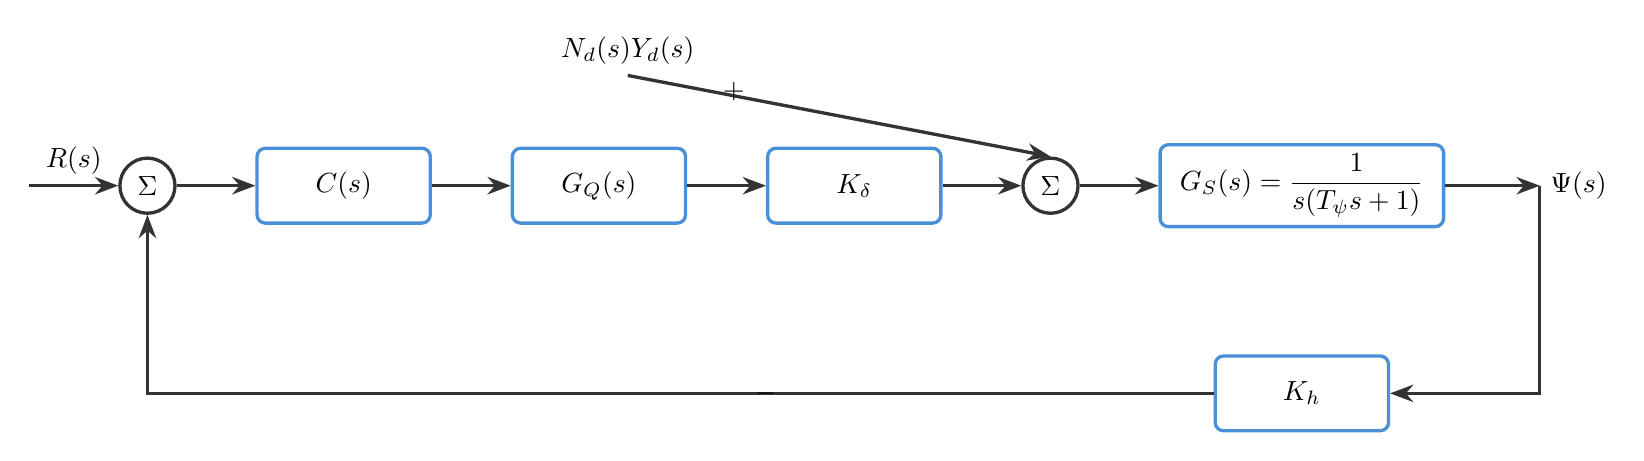
\begin{tikzpicture}[
  >=Stealth,
  line width=1.2pt,
  block/.style={rectangle, draw=blockblue, rounded corners=3pt, minimum width=2.2cm, minimum height=0.95cm, align=center},
  sum/.style={circle, draw=linegray, minimum size=0.7cm},
  flow/.style={->, draw=linegray, line width=1.2pt}
]
  \node[sum] (s1) at (0,0) {$\Sigma$};
  \node[block, right=1.0cm of s1] (ctrl) {$C(s)$};
  \node[block, right=1.0cm of ctrl] (servo) {$G_Q(s)$};
  \node[block, right=1.0cm of servo] (kd) {$K_\delta$};
  \node[sum, right=1.0cm of kd] (s2) {$\Sigma$};
  \node[block, right=1.0cm of s2, minimum width=3.6cm] (ship) {$G_S(s)=\dfrac{1}{s(T_\psi s+1)}$};
  \node[block, below=1.6cm of ship] (kh) {$K_h$};
  \coordinate (out) at ($(ship.east)+(1.2,0)$);

  \draw[flow] (-1.5,0) -- node[above] {$R(s)$} (s1);
  \draw[flow] (s1) -- (ctrl);
  \draw[flow] (ctrl) -- (servo);
  \draw[flow] (servo) -- (kd);
  \draw[flow] (kd) -- (s2);
  \draw[flow] (s2) -- (ship);
  \draw[flow] (ship) -- (out) node[right] {$\Psi(s)$};

  \draw[flow] (out) |- (kh);
  \draw[flow] (kh.west) -| node[pos=0.2,left] {$-$} (s1.south);

  \draw[flow] (6.1,1.4) -- (s2.north) node[pos=0.2,right] {$+$};
  \node[above] at (6.1,1.4) {$N_d(s)Y_d(s)$};
\end{tikzpicture}
\end{document}
